\section*{Dati e risultati}

Per ogni resistenza a nostra disposizione abbiamo effettuato una misura volt-amperometrica con entrambi i circuiti realizzati. Pertanto per ognuna delle resistenze abbiamo due coppie di valori di corrente e tensione $(I\ped{x}, V\ped{x})$.
Quindi grazie ai valori acquisiti possiamo determinare il valore sperimentale delle resistenze, sempre sfruttando la legge integrale di Ohm, poichè le resistenze sono componenti circuitali Ohmici.

\begin{equation}
	\text{Amperomero a monte:} \qquad R\ped{x} \,=\, \frac{V\,R\ped{v}}{R\ped{v}\,I\,-\,V}
\end{equation}
\begin{equation}
	\text{Amperomero a valle:} \qquad R\ped{x} \,=\, \frac{V\,-\,I\,R\ped{a}}{I}
\end{equation}
%
dove $R\ped{x}$ indica il valore della resistenza da stimare, $V$ è la differenza di potenziale misurata con il voltometro, $R\ped{v}$ è la resistenza interna del voltometro, $R\ped{a}$ è la resistenza interna dell'amperometro e $I$ è il valore di corrente misurato grazie all'amperometro.

Inoltre per avere un riscontro che i dati ottenuti siano affidabili abbiamo misurato il valore delle varie resistenze mediante il multimetro digitale. In questo modo potremo osservare se ci sono delle discrepanze rilevanti tra il valore teorico e quello sperimentale delle resistenze. Di seguito sono tabulati i risultati ottenuti.

\begin{table}[h]
  \centering
  \small
  \begin{tabular}{l | c c}
      \multicolumn{3}{c}{\textbf{Resistenze [$\Omega$]}} \\
      \toprule
      Valori ``veri'' & Monte & Valle \\
      \midrule
      983 k   & (1000 $\pm$ 30) k & (1000 $\pm$ 20) k \\
      99.83 k & (98.0 $\pm$ 1.7) k & (99.4 $\pm$ 1.6) k \\
      9937 & 10100 $\pm$ 170 & 9940 $\pm$ 160 \\
      999    & 1010 $\pm$ 20 & 1000 $\pm$ 20 \\
      98.88  & 99 $\pm$ 2 & 99 $\pm$ 2 \\
      9.97   & 10.3 $\pm$ 0.3 & 5.3 $\pm$ 0.3 \\
      1.04   & 0.95 $\pm$ 0.06 & 1.71 $\pm$ 0.08 \\
      \bottomrule
  \end{tabular}
\end{table}


Infine abbiamo misurato il valore della resistenza di una lampadina, in grado di sopportate una differenza di potenziale massima di $12\,\si{\volt}$, prendendo una serie di misure volt-amperometriche utilizzando entrambi i circuiti a nostra disposizione.
Anche in questo caso abbiamo graficato i dati e abbiamo ottenuto il seguente risultato:

\begin{SCfigure}[0.6][hbtp]
        \centering
        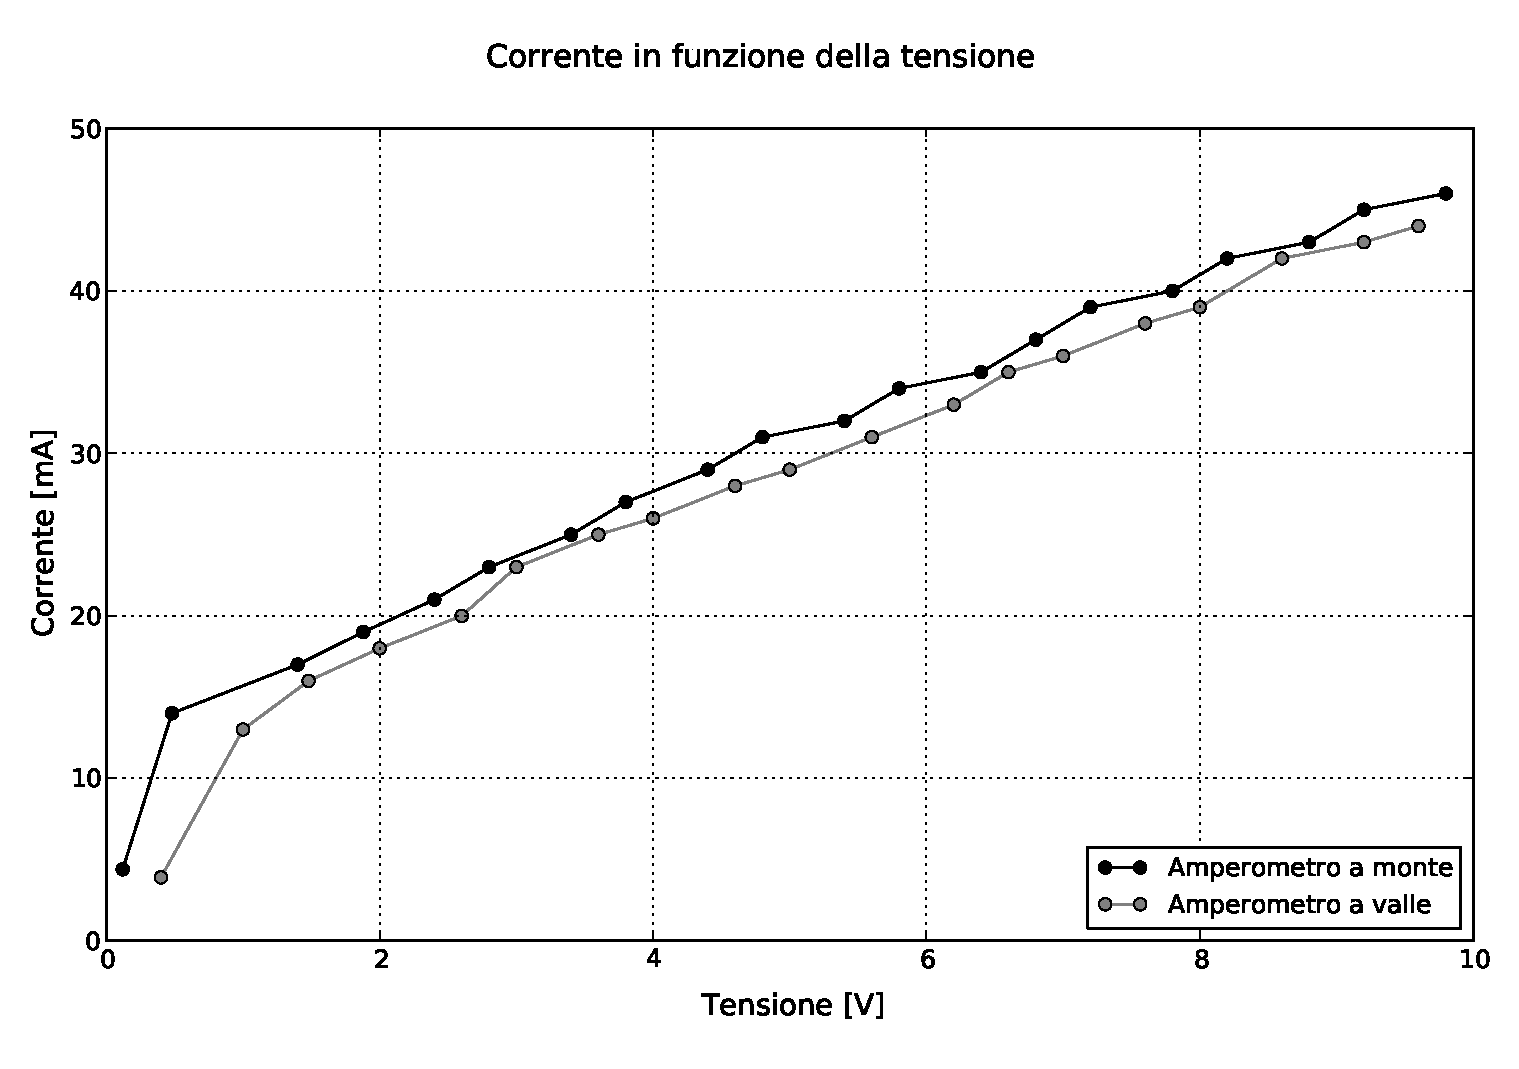
\includegraphics[scale=0.50]{lampadina.pdf}
        \caption{Questo grafico illustra la relazione che sussiste tra la corrente che attraversa la lampadina e la differenza di potenziale ai capi della resistenza interna della stessa. I due set di misure fanno riferimento ai due circuiti utilizzati per acquisire i valori graficati. Le incertezze sui dati non sono visibili in quanto molto piccole rispetto alle scale utilizzate. Come si può notare l'andamento non è lineare, soprattutto per valori piccoli di tensione, questo è giustificato dal fatto che la resistenza della lampadina non è un elemento circuitale Ohmico.}
\end{SCfigure}

